\section{Hairball Plugins} \locallabel{sec:plugins}
In this section, we describe four Hairball plugins written to perform
\sprogram{} static analysis.  The plugins were designed to analyze \sprogram{s}
submitted as part of our two-week interdisciplinary Animal Tlatoque summer
camp~\cite{Franklin:2013:SBO}. The plugins target the computer science concepts
used in the camp's cumulative assignment, an interactive movie about an
animal. For this assignment, students were to demonstrate state initialization,
use of \broadcast{} and \receive{} blocks, synchronization between \say{} and
\playsound{} blocks, and creation of complex animation. While these plugins
were developed for our summer camp, each provides valuable feedback that is
generally useful both as a lint-like tool for individual developers of
\sprogram{s} and for others who are tasked with analyzing numerous
\sprogram{s}.

Each Hairball plugin for the camp was designed to evaluate whether, or to what
extent, the \sprogram{} demonstrated competence in an area. More precisely,
these plugins were designed to discover instances of the aforementioned
concepts contained within a \sprogram{} and label each instance as \correct{},
\semincor{}, \incor{}, or \incom{}. Instances labeled \correct{} should
indicate that the concept was implemented correctly. Instances labeled
\semincor{} should indicate that the concept was implemented in a way that may
not always work when executed. Instances labeled \incor{} should indicate the
concept was implemented incorrectly. Finally, instances labeled \incom{} should
indicate that only a subset of the required blocks for a concept was
discovered. A single \sprogram{} may contain multiple instances of a concept
distributed across any or all of the labels. Ideally, instances labeled
\correct{} should not require manual analysis, whereas instances with any other
label should be inspected manually.


\subsubsection{Initial State}
In any program, correctly setting the initial state is important.  In
\sprogram{s}, the significance is different.  \sprogram{s} are comprised of
animations, and in the runtime environment, they may run from start to finish
and be restarted again.  Alternatively, they may be stopped in the middle and
restarted again.  We want to determine via static analysis whether the code
runs the same way in these two events.

The first problem is where to start the analysis.  In traditional programs,
execution starts at \emph{main}. However, \sprogram{s} have no such globally
defined starting point. Therefore, we taught our students to start their
\sprogram{} using the green flag button. Thus the starting point for our
evaluation is the \greenflag{} block.

The most complex problem, and the problem that introduces the possibility of
error into our analysis, is that sprites are placed on the stage during
implementation thus giving them an implicit set of attributes, which we will
refer to as the base attributes. Explicit initialization for a particular
attribute, e.g., position or orientation, is only required when that attribute
is modified by a script of the \sprogram{}. Thus, the challenge is
distinguishing segments of scripts that perform initialization from those that
perform general modification. To discover instances of initialization, we first
determine the set of blocks that can be considered initialization blocks and
then we restrict the location within the scripts that we search for these
blocks. We call this location the \initzone{}.

\begin{table}
\centering
\begin{tabular}{|c|c|c|} \hline
Category & Relative&Absolute\\ \hline \hline
Costume& next costume & switch to costume x\\ \hline
Visibility& & show/hide\\ \hline
Orientation&turn clockwise x degrees&point in direction x\\ \hline
Position&move x steps & go to x,y\\ \hline
Size&change size by x\% & set size to x\%\\ \hline
Background&next background & switch to background x\\ \hline
\end{tabular}
\caption{Lists the five categories of initial state, and provides a subset of
  the \rel{} and \abs{} modification blocks for each category.}
\locallabel{table:initialstate}
\end{table}

Attribute modifying Scratch blocks can be labeled as \rel{} or
\abs{}. \emph{Relative} Scratch blocks alter the attribute based upon its
current value, whereas \abs{} Scratch blocks directly set the attribute. As
such, only \abs{} blocks can be considered initialization
blocks. Table~\localref{table:initialstate} shows our categorization for a
subset of attribute modifying Scratch blocks.

For an \abs{} block to be considered an initialization block, it must appear in
the \initzone{}. We define the \initzone{} only for scripts beginning with a
\greenflag{} block. The \initzone{} begins at the start of the script and ends
when either a \rel{} block or a \broadcast{} block is encountered. We take a
conservative approach when encountering blocks contained within loops or
conditionals---\abs{} blocks are ignored due to the possibility that the block
is not executed, and \rel{} blocks continue to signify the end of the
\initzone{} due to the possibility that the block is executed.

The initialization plugin labels a modified attribute of a sprite as \correct{}
when an \abs{} block for the same attribute exists in the
\initzone{}. Instances are labeled as \incor{} otherwise. Non-modified
attributes are ignored. Finally, despite this plugin's ability to detect
unnecessary initialization, we did not include it as part of our analysis.


\subsubsection{Say and Sound Synchronization}
Synchronization between a speech bubble (\say{} block) and sound file
(\playsound{} block) is not straightforward in Scratch. The desired behavior is
that whenever a speech bubble appears with a message, a sound file of a voice
speaking the message plays. When the sound is complete, the speech bubble
disappears.

Achieving this effect is complicated by the timing semantics of the two forms
of the \say{} block, and the two forms of the \playsound{} block in Scratch.
One form of the \say{} block places the speech bubble on the screen
indefinitely (until replaced by another \say{} block, or \emph{erased} with an
empty \say{} block), while the other, \sayfor{}, puts a speech bubble on the
screen for $n$ seconds and, as a side-effect, delays execution of the script
for $n$ seconds. Similarly, there are two forms of the block for playing a
sound clip: \playsounddone{} plays the entire sound file before continuing
execution of the script, while \playsound{} starts playing the sound and
immediately continues with the script execution.

\begin{figure}[!t]
\centering
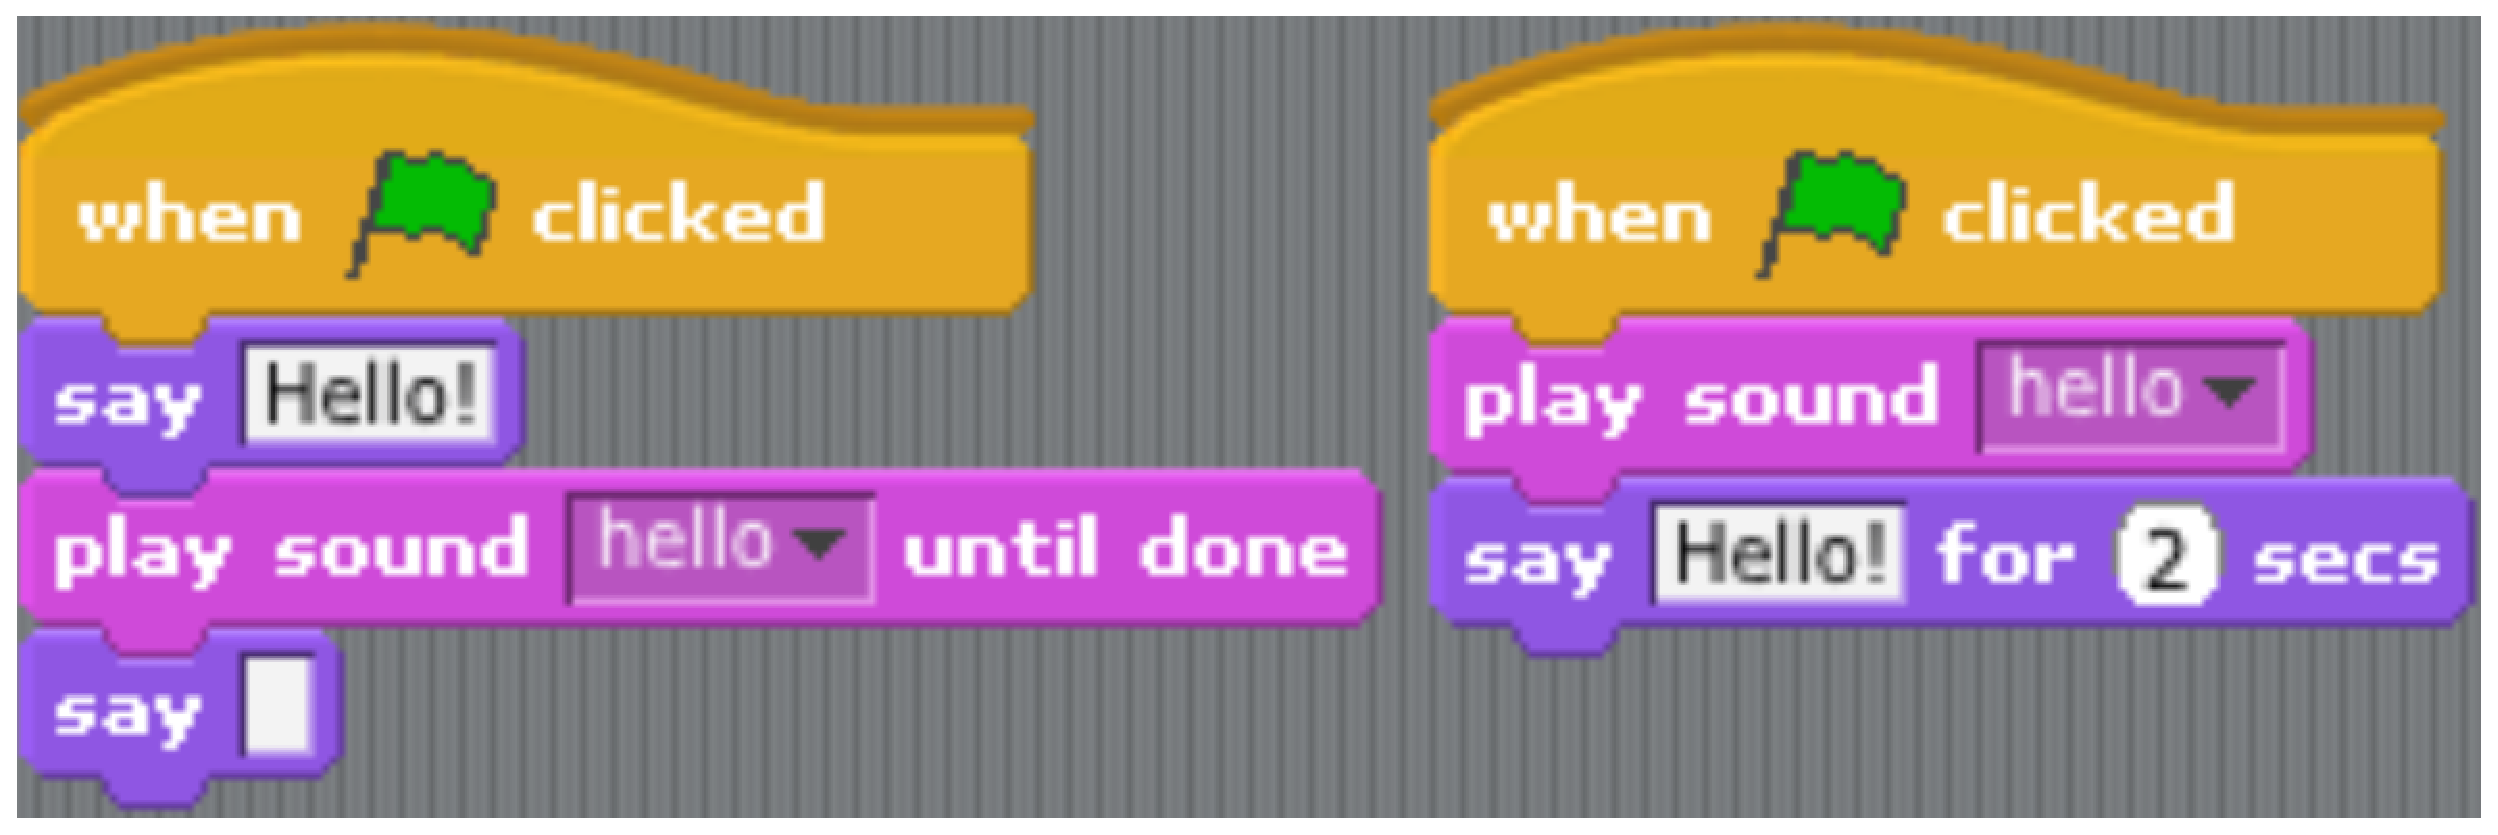
\includegraphics[width=5.25in]{graphs/saysound.eps}
\caption{Shows the two methods for synchronizing messages from the \say{}
  blocks with sound files played through the \playsound{} blocks. While both
  methods can produce the desired effect, the method on the right requires
  manually setting an appropriate duration in the \sayfor{} block and thus is
  not as robust to modifications, whereas the method on the left guarantees
  synchronization between the play of the sound file and the display of the
  message.}  \locallabel{fig:saysound}
\end{figure}

Figure~\localref{fig:saysound} depicts the two methods to produce the desired
effect. The first, displayed on the right, is to asynchronously play the sound
via the \playsound{} block followed by a \sayfor{} block with duration equal to
the elapsed time of the sound. Unfortunately, the timing must be manually
determined and needs to be updated whenever the sound file changes. The second,
displayed on the left, is to use a \say{} block to display the message,
followed by a \playsounddone{} block, ending with an empty \say{} block to
remove the speech bubble. The campers were taught the latter method as the
correct approach because it is robust to modifications of both the sound file,
and to the message in the \say{} block.

Thus the say and sound synchronization plugin detects instances of this concept
by looking for sequential \say{} and \playsound{} blocks and verifies the
instances are implemented using the appropriate method.  A \correct{} instance
contains the previously described three blocks in the proper order.  Instances
following the method requiring manual timing are labeled \semincor{}. Instances
that have both \say{} and \playsound{} blocks, but do not match either of these
methods are labeled \incor{}, and isolated uses of \say{} or \playsound{}
blocks are labeled \incom{}.


\subsubsection{Broadcast and Receive}
One use of Scratch's \broadcast{} blocks is to trigger the execution of other
sprites' scripts beginning with the appropriate \receive{} block. We taught our
campers the broadcast and receive concept in the context of two animal sprites
conversing, where each sprite would signal the other's turn via an event
broadcast. In the camp's cumulative assignment, the campers demonstrated an
understanding of the broadcast and receive concept by transferring this idea to
the new context of triggering scene changes in their interactive movie.

The broadcast and receive plugin verifies that for each broadcast or receive
event, there is a \broadcast{} block and at least one corresponding \receive{}
block. Such instances are labeled \correct{}. All instances with a \broadcast{}
block appearing in the same script with another instance's \broadcast{} block
are labeled as \semincor{}. All other instances are labeled \incom{}. Note that
this plugin does not use the \incor{} label.

\subsubsection{Complex Animation}
We have a very specific definition of the term \emph{complex animation} for the
purpose of our assessment.  We use this term to refer to animation involving
integration of costumes, motion, timing, and repetition control structures such
as loops. This definition of complex animation is to distinguish from, for
example, the \glideto{} block built into Scratch.  One example of complex
animation is realistic motion of sprites representing people and animals, e.g.,
people walking, birds flying, and snakes slithering.  Creating these complex
animations requires the correct integration of several computer science
concepts. For example, creating an animation sequence where a sprite spins
around, requires integration of loops, rotation, and timing.

A necessary component of complex animation instances is the pairing of costume
change blocks with either rotation blocks, or motion blocks. We define a
complex animation instance as either a loop containing these necessary
components or a repeated sequence of these necessary components, since a
repeated sequence can be considered an unrolled loop. In order to be labeled
\correct{}, an instance must also make use of a Scratch block that introduces a
delay; otherwise the instance is labeled \semincor{}. The plugin additionally
labels instances that use repeated sequences instead of loops as \semincor{}
because the student did not demonstrate competence in the computer science
concept of loops. Finally, if the \sprogram{} is missing any critical element,
e.g., repetition, it is labeled \incom{}.
